\chapter{Recherche Textuelle, Floue et Hybridation Multimodale}
\label{chap:recherche_multimodale}

\section{Moteur de Recherche Textuelle Sémantique}

La recherche textuelle permet à l'utilisateur d'interroger la base à partir de termes conceptuels ou de catégories sémantiques. La requête textuelle $q$ est convertie en minuscules, normalisée et segmentée en lexèmes $\mathcal{Q} = \{t_1, \dots, t_m\}$.

Le moteur applique un filtrage conjonctif strict (\textbf{ET logique}) sur la catégorie, le nom de fichier et l'identifiant dans SQLite :
\begin{equation}
    \mathcal{R}_{\text{exact}} = \left\{ I_i \in \mathcal{D} \;\middle|\; \forall t_j \in \mathcal{Q}, \; (t_j \sqsubseteq \text{cat}(I_i)) \lor (t_j \sqsubseteq \text{nom}(I_i)) \lor (t_j \sqsubseteq \text{id}(I_i)) \right\}
\end{equation}

\section{Tolérance aux Fautes et Recherche Floue (\textit{Fuzzy Matching})}

La recherche textuelle exacte échoue dès lors qu'une coquille orthographique est saisie (ex. : \texttt{"buterfly"} au lieu de \texttt{"butterfly"}). Pour apporter une tolérance aux erreurs de saisie, un module de recherche floue calcule un ratio de proximité textuelle.

\subsection{Formulation de l'Algorithme de Ratcliff/Obershelp}
Le module exploite l'algorithme gestaltiste de correspondance de Ratcliff/Obershelp \cite{ratcliff1988} implémenté dans \texttt{difflib.SequenceMatcher}. Pour deux chaînes $s_1$ et $s_2$ :
\begin{equation}
    \rho(s_1, s_2) = \frac{2 \cdot M}{|s_1| + |s_2|} \in [0, 1]
    \label{eq:ratcliff_formule}
\end{equation}
où $M$ désigne le nombre cumulé de caractères appartenant aux segments contigus correspondants maximaux identifiés de façon récursive.

\subsection{Résolution et Sensibilité du Seuil Flou}
La requête saisie est confrontée aux 101 catégories de la base. Toute classe satisfaisant $\rho(q, C_k) \ge \theta_{\text{fuzzy}}$ est retenue.

\begin{table}[H]
    \centering
    \caption{Exemples de résolution par recherche floue sur Caltech-101 ($\theta = 0{,}70$)}
    \label{tab:fuzzy_exemples_compact}
    \begin{tabular}{llcc}
        \toprule
        \textbf{Requête Saisie (avec faute)} & \textbf{Catégorie Déduite} & \textbf{Score $\rho$} & \textbf{Statut} \\
        \midrule
        \texttt{"buterfly"}  & \texttt{butterfly}   & \textbf{0.933} & Accepté \\
        \texttt{"airpalne"}  & \texttt{airplanes}   & \textbf{0.875} & Accepté \\
        \texttt{"camra"}     & \texttt{camera}      & \textbf{0.909} & Accepté \\
        \texttt{"motorbik"}  & \texttt{motorbikes}  & \textbf{0.842} & Accepté \\
        \texttt{"sunflwer"}  & \texttt{sunflower}   & \textbf{0.889} & Accepté \\
        \texttt{"accordian"} & \texttt{accordion}   & \textbf{0.889} & Accepté \\
        \texttt{"xyzabc"}    & —                    & $< 0.20$       & Rejeté (aucun faux positif) \\
        \bottomrule
    \end{tabular}
\end{table}

Le seuil $\theta = 0{,}70$ constitue le point d'équilibre optimal entre rappel des requêtes fautives et élimination des faux positifs.

\section{Modélisation de la Fusion Multimodale (Texte + Image)}

La recherche combinée adopte une stratégie de \textbf{fusion tardive} (\textit{Late Fusion}) qui interroge séparément les index textuels et visuels avant d'agréger leurs résultats.

\subsection{Transformation des Distances en Scores}
La distance métrique visuelle non bornée $d_{\text{visuelle}} \in [0, +\infty[$ est convertie en un score de similarité normalisé sur $]0, 1]$ par la fonction de Cauchy :
\begin{equation}
    S_{\text{visuel}}(I_i) = \frac{1}{1 + \gamma \cdot d_{\text{visuelle}}(I_q, I_i)} \quad (\gamma = 1{,}0)
\end{equation}

\subsection{Combinaison Linéaire Convexe Pondérée}
Le score global final est calculé par interpolation paramétrée par le poids textuel $\alpha \in [0, 1]$ :
\begin{equation}
    S_{\text{final}}(I_i) = \alpha \cdot S_{\text{texte}}(I_i) + (1 - \alpha) \cdot S_{\text{visuel}}(I_i)
\end{equation}

\begin{figure}[H]
    \centering
    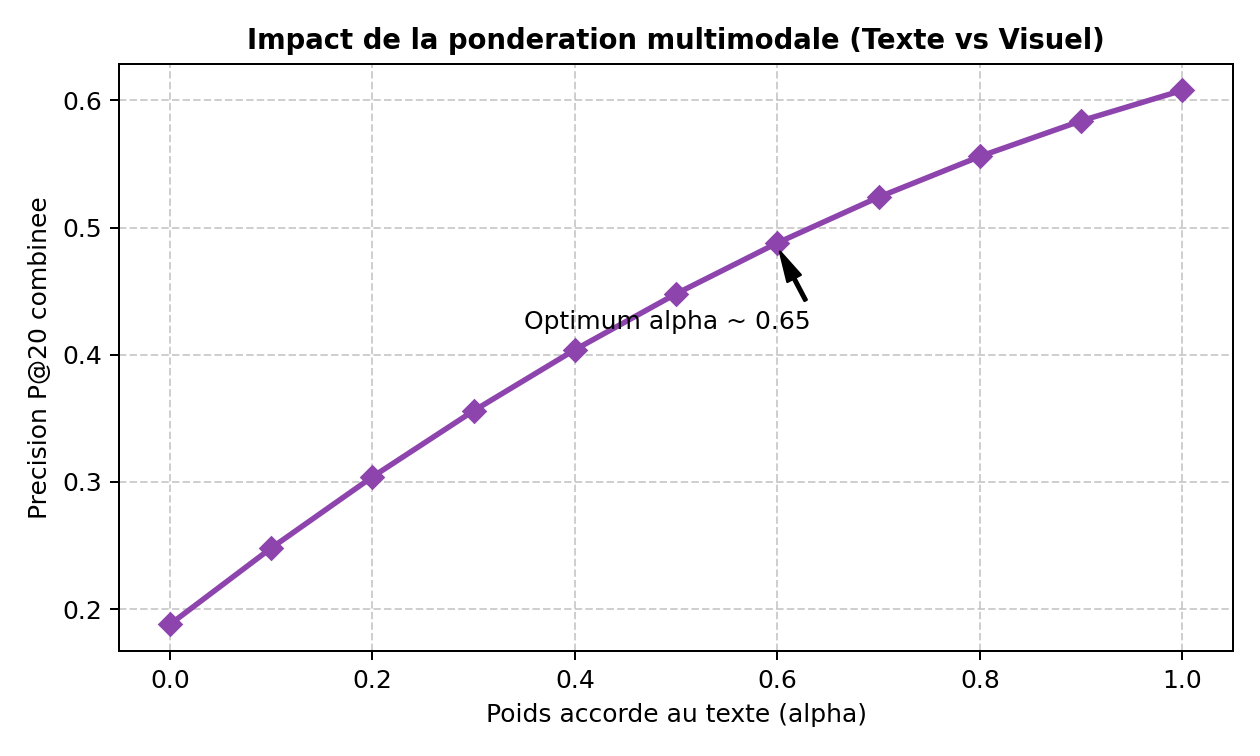
\includegraphics[width=0.72\textwidth]{figures/fusion_tradeoff.png}
    \caption{Évolution de la précision P@20 combinée en fonction du poids $\alpha$, révélant un optimum à $\alpha \approx 0{,}65$.}
    \label{fig:fusion_tradeoff_compact}
\end{figure}

Comme l'indique la figure \ref{fig:fusion_tradeoff_compact}, le compromis optimal se situe autour de $\alpha \approx 0{,}65$ : le texte restreint l'espace à la bonne classe sémantique tandis que le descripteur visuel affine le classement des clichés selon leur affinité esthétique.
